\documentclass[11pt]{beamer}
\usetheme{simple}
\setbeamertemplate{footline}{} 
\usepackage{tikz}
\usepackage[T1]{fontenc}
\usepackage{lmodern}
\usepackage{pgfplots}
\usepackage{amsmath, amssymb, amsthm}   
\pgfplotsset{
        % declare the function you want to plot so you can reuse it easily later
        /pgf/declare function={
            T1(\u)=ln(0.5*(-2*\u+sqrt(4+4*\u^2)));
            T0(\u)=ln(0.5*(2*\u+sqrt(44+4*\u^2)));     
            U0(\u)=\u-1;
            T12(\u)=ln(-1-2*\u);
        },
        % define style to use for the plot to draw only ticks at `\myxlist'
        % (the plot should be invisible)
        my ticks/.style={
            samples at={\myxlist},
            mark=none,
            draw=none,
%            only marks,     % <-- uncomment me to show the data points
        },
every non boxed y axis/.append style={y axis line style=-}
    }
%\pgfplotsset{ every non boxed y axis/.append style={y axis line style=-}}
\setbeamertemplate{navigation symbols}{}
\begin{document}
\begin{frame}


\tikzset{every picture/.style={line width=0.75pt}} %set default line width to 0.75pt        

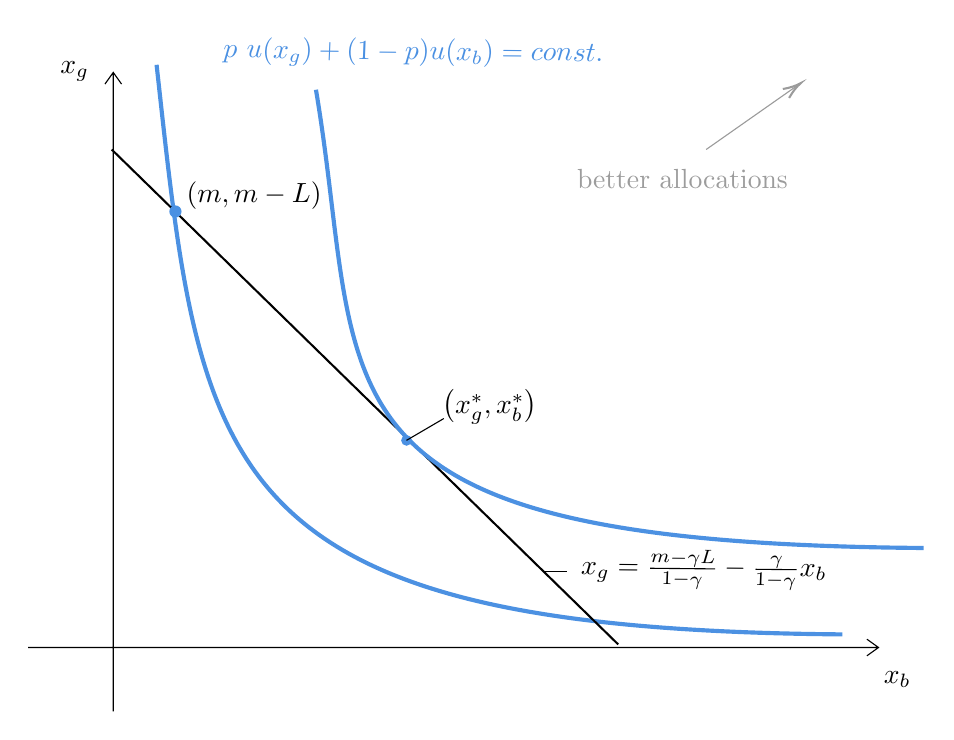
\begin{tikzpicture}[x=0.75pt,y=0.75pt,yscale=-.8,xscale=.8]
%uncomment if require: \path (0,443); %set diagram left start at 0, and has height of 443

%Shape: Axis 2D [id:dp3991482376662687] 
\draw  (74,382.93) -- (586.09,382.93)(125.21,36.6) -- (125.21,421.41) (579.09,377.93) -- (586.09,382.93) -- (579.09,387.93) (120.21,43.6) -- (125.21,36.6) -- (130.21,43.6)  ;
%Curve Lines [id:da07640526755648236] 
\draw [color={rgb, 255:red, 74; green, 144; blue, 226 }  ,draw opacity=0.99 ][line width=1.5]    (151.3,32) .. controls (178.3,276) and (182.28,372.03) .. (564.28,375.03) ;


%Straight Lines [id:da1654344051931811] 
\draw [line width=0.75]    (124.28,83.03) -- (429.28,381.03) ;


%Straight Lines [id:da7552857580314549] 
\draw [color={rgb, 255:red, 155; green, 155; blue, 155 }  ,draw opacity=1 ]   (482.3,83) -- (537.66,44.15) ;
\draw [shift={(539.3,43)}, rotate = 504.94] [color={rgb, 255:red, 155; green, 155; blue, 155 }  ,draw opacity=1 ][line width=0.75]    (10.93,-3.29) .. controls (6.95,-1.4) and (3.31,-0.3) .. (0,0) .. controls (3.31,0.3) and (6.95,1.4) .. (10.93,3.29)   ;

%Shape: Circle [id:dp6490632364348066] 
\draw  [draw opacity=0][fill={rgb, 255:red, 74; green, 144; blue, 226 }  ,fill opacity=1 ] (158.97,120.35) .. controls (158.97,118.32) and (160.61,116.67) .. (162.65,116.67) .. controls (164.68,116.67) and (166.33,118.32) .. (166.33,120.35) .. controls (166.33,122.39) and (164.68,124.03) .. (162.65,124.03) .. controls (160.61,124.03) and (158.97,122.39) .. (158.97,120.35) -- cycle ;
%Curve Lines [id:da28778278460477735] 
\draw [color={rgb, 255:red, 74; green, 144; blue, 226 }  ,draw opacity=0.99 ][line width=1.5]    (247.28,47.03) .. controls (278.28,231.03) and (231.3,320) .. (613.3,323) ;


%Shape: Circle [id:dp5978063302390677] 
\draw  [draw opacity=0][fill={rgb, 255:red, 74; green, 144; blue, 226 }  ,fill opacity=1 ] (298.56,258.18) .. controls (298.56,256.38) and (300.02,254.93) .. (301.82,254.93) .. controls (303.62,254.93) and (305.07,256.38) .. (305.07,258.18) .. controls (305.07,259.98) and (303.62,261.44) .. (301.82,261.44) .. controls (300.02,261.44) and (298.56,259.98) .. (298.56,258.18) -- cycle ;
%Straight Lines [id:da8727541988151988] 
\draw    (385.28,337.03) -- (398.28,337.03) ;


%Straight Lines [id:da7889466398132292] 
\draw    (301.82,258.18) -- (324.28,245.03) ;



% Text Node
\draw (597.35,402.33) node   {$x_{b}$};
% Text Node
\draw (210,111) node   {$( m,m-L)$};
% Text Node
\draw (102,36) node   {$x_{g}$};
% Text Node
\draw (468,101) node  [align=left] {\textcolor[rgb]{0.61,0.61,0.61}{better allocations}};
% Text Node
\draw (481,336) node [rotate=-0.56,xslant=0.03]  {$x_{g} =\frac{m-\gamma L}{1-\gamma } -\frac{\gamma }{1-\gamma } x_{b}$};
% Text Node
\draw (306,25) node [color={rgb, 255:red, 74; green, 144; blue, 226 }  ,opacity=1 ,rotate=-0.56,xslant=0.03]  {$p\ u( x_{g}) +( 1-p) u( x_{b}) =const.$};
% Text Node
\draw (352,238) node   {$\left( x^{*}_{g} ,x^{*}_{b}\right)$};


\end{tikzpicture}


\end{frame}
\end{document}